%$Id: config_nux.tex 145 2005-03-25 08:26:35Z myk $

\bghdr{images/fond-nux}



%\begin{center}
%
\includegraphics{images/logo_Linux}
%\end{center}

\subsection{Configuration sous Linux}

\subsubsection{Configuration IP}
Tu as besoin de conna\^itre ton adresse IP, ton masque de sous-r\'eseau et ta  passerelle. Toutes les informations se trouvent page \pageref{calcul_ip}. Bien s\^ur, pour  l'ensemble des manipulations d\'ecrites ci-dessous tu auras besoin de ton  mot de passe super-utilisateur (\emph{root}) !

\paragraph{Sous Ubuntu/Kubuntu}
\label{Ubuntu:IP}
Il existe deux mani\`eres de configurer tes param\`etres r\'eseaux: l'une utilise les outils graphiques de l'environnement que tu as choisi (Gnome ou KDE), 
l'autre utilise simplement la ligne de commande. Bien sûr, les outils graphiques ne sont qu'un interm\'ediaire modifiant les fichiers dont on te parle 
plus bas. Ils te permettent parfois d'enregistrer une configuration r\'eseau, ce qui facilite la gestion si tu rentres souvent chez toi. Pour obtenir le 
m\^eme r\'esultat en ligne de commande il faut utiliser un script.
\begin{description}
\item[\'Etape 1 : configuration de la connexion au r\'eseau] \
 
\begin{itemize}
\item Va dans \menu{Syst\`eme}, \menu{Pr\'ef\'erences} puis \menu{Connexions r\'eseau}.
\item Dans l'onglet \menu{Filaire}, clique sur \menu{Ajouter}.
\item Compl\`ete le champ \menu{Nom de la connexion}  par ce que tu veux ; "Casert de Polytechnique" par exemple.
\item Puis va dans l'onglet \menu{Param\`etres IPv4}.
\item S\'electionne la m\'ethode \menu{Manuel}.
\item Clique sur \menu{Ajouter}, puis remplis les champs \menu{Adresse}, \menu{Masque de r\'eseau} et  \menu{Passerelle} par les donn\'ees qui te sont propres. 
\item Compl\`ete le  champ \menu{Serveurs DNS} par \server{129.104.201.53, 129.104.201.51} et le champ \menu{Domaines de recherche} par \server{eleves.polytechnique.fr, polytechnique.fr}. 
\item Coche enfin l'option \menu{Disponible pour tous les utilisateurs}, clique sur \menu{Appliquer} et enfin rentre ton mot de passe super-utilisateur (root).
\end{itemize}

\item[\'Etape 2 : configuration du proxy (= serveur mandataire)] \
\begin{itemize}
\item Va  dans \menu{Param\`etres Syst\`eme}, \menu{R\'eseau} puis \menu{Serveur Mandataire}.
\item S\'electionne  la \menu{M\'ethode} \menu{Automatique}.
\item Compl\`ete le champ  \menu{URL de configuration} par \urllink{http://config/proxy.pac}. 
\item Clique sur \menu{Appliquer à tout le syst\`eme...} et rentre ton mot de passe super-utilisateur si on te le demande.
\end{itemize}

\item[\'Etape 3 (\'eventuellement)] \
\begin{itemize}
\item Clique  sur l'ic\^one de l'applet R\'eseau dans la zone de notification, en forme  de fl\`eches t\^ete-b\^eche ou d'ondes. S\'electionne le r\'eseau que tu as  configur\'e dans la 1\`ere \'etape, et te voilà connect\'e à Internet !
\item Une fois ta configuration r\'eseau termin\'ee, tu peux la tester en \emph{pinguant} \fkz (dans une console), o\`u tu devrais voir quelque chose comme :
\end{itemize}

\cmdline{\$ ping frankiz\\
PING frankiz.eleves.polytechnique.fr (129.104.201.51) 56(84) bytes of data.\\
64 bytes from Frankiz.eleves.polytechnique.fr ...}

\end{description}

\label{ubuntu_mirror}

\subsubsection{Configuration du gestionnaire de paquets}

Il faut d\'esormais configurer le gestionnaire de paquets pour qu'il utilise les miroirs du BR et non les miroirs à l'ext\'erieur du campus, qui sont plus lents. \
Va  dans \menu{Applications}, \menu{Logith\`eque Ubuntu} puis menu \menu{\'edition}, \menu{Sources de logiciels...}. 
Entre ton  mot de passe super-utilisateur puis s\'electionne l'onglet \menu{Autres  logiciels}. 
D\'ecoche les cases comprenant une adresse du type \urllink{http://archive.canonical.com/ubuntu version}, o\`u \textit{version} correspond à la version d'Ubuntu install\'ee sur ton ordinateur. 
À l'impression de l'InfoBR, la version actuelle est \textbf{oneiric} et la pr\'ec\'edente est \textbf{natty}. \
Clique sur \menu{Ajouter}, puis entre dans le champ \menu{Ligne APT} :
\cmdline{deb ftp://miroir/linux/ubuntu version main restricted universe multiverse}
Tu auras bien s\^ur remplac\'e \textit{version} par ta version d'Ubuntu (\textit{maverick}/\textit{lucid}/\textit{karmic}/...). \\
Clique ensuite sur \menu{Ajouter une source de mise à jour}. Fais de même pour les lignes suivantes :
\cmdline{deb ftp://miroir/linux/ubuntu version-updates main restricted universe  multiverse \\
deb ftp://miroir/linux/ubuntu version-security main restricted universe  multiverse}
Tu peux aussi utiliser le d\'ep\^ot suivant mais attention il contient des logiciels non support\'es par Canonical, l'\'equipe de d\'eveloppement d'Ubuntu (en particulier il peut arriver que certains logiciels contiennent des erreurs) :
\cmdline{deb ftp://miroir/linux/ubuntu version-backports main restricted universe multiverse}
Le  BLL (Binet Logiciels Libres) dispose par ailleurs d'un miroir  non-officiel qui contient des paquets (flash, ...) non  inclus dans la distribution de base pour diverses raisons, en paticulier l\'egales ou \'ethiques. Pour en profiter, rajoute aussi la ligne :
\cmdline{deb ftp://miroir/linux/bll version main}
Clique enfin sur \menu{Fermer} puis r\'eponds \menu{Actualiser} à la fenêtre de dialogue qui appara\^it. \\

Note : il n'est pas n\'ecessaire de configurer Synaptic dans ses Pr\'ef\'erences pour y sp\'ecifier un proxy quelconque.

\subsubsection{Configuration antivirus}

{C'est pas non plus comme si y'en avait besoin \dots}

%\subsubsection{Configuration du pare-feu}
%
%La solution la plus simple pour se faire un \emph{firewall} sous linux est d'utiliser les \emph{iptables}. Pour ceci la premi\`ere \'etape est
%d'installer le paquet \app{iptables} pour ta distribution. Pour savoir comment configurer ton \emph{firewall} pour le r\'eseau de l'X, consulte le Wikix.

\subsubsection{Configuration navigateur web}

\flimage{images/nux_firefox_icon}{0.12}{l} Le BR te conseille d'utiliser \app{Firefox} ou
\app{Konqueror} (le navigateur fourni par d\'efaut avec KDE). Dans tous les cas, la seule
configuration \`a  effectuer est celle du serveur mandataire.

Pour \app{Firefox}, il suffit d'aller dans \menu{\'Edition}, \menu{Pr\'ef\'erences} et dans l'onglet \menu{Avanc\'e}, puis de cliquer sur l'onglet
\menu{R\'eseau}, et enfin \menu{Param\`etres de connexion} ; ensuite coche la case \menu{Adresse de configuration automatique du proxy}, et rentre 
\urllink{http://config/proxy.pac}.

Sous \app{Konqueror}, cela se trouve dans le menu \menu{Configuration}, \menu{Configurer Konqueror},
dans l'onglet \menu{Serveur mandataire}. \emph{Attention}: si tu ne configures pas le serveur mandataire dans Konqueror,
les logiciels KDE (\app{KGet}, \app{Adept},\dots) ne l'utiliseront pas!

Pour \app{Google Chrome}, la configuration se règle automatique sur celle du système. Tu n'as donc rien à faire si le reste est correctement configuré.

\imagepos{images/nux_proxy_firefox}{0.65}{Configuration du serveur mandataire sous Firefox}{ht}

\pagebreak

\subsubsection{Configuration \emph{mail}}

\flimage{images/nux_kmail_icon}{0.12}{l} Les clients \emph{mail} les plus
utilis\'es sont \app{Kmail} et \app{Thunderbird}. La configuration est semblable, quel que soit le
client utilis\'e.

Pour \app{Kmail}, va dans \menu{Configuration}, \menu{Configurer Kmail}. Choisis la
rubrique \menu{Comptes}. Commence par cr\'eer un nouveau compte dans
l'onglet \menu{R\'eception des messages} en cliquant sur le bouton
\menu{Ajouter\ldots} et choisis le type POP3.


\noindent
  \begin{figure*}[!h]
    \begin{center}  
      \subfloat[R\'eception des messages]{ 
      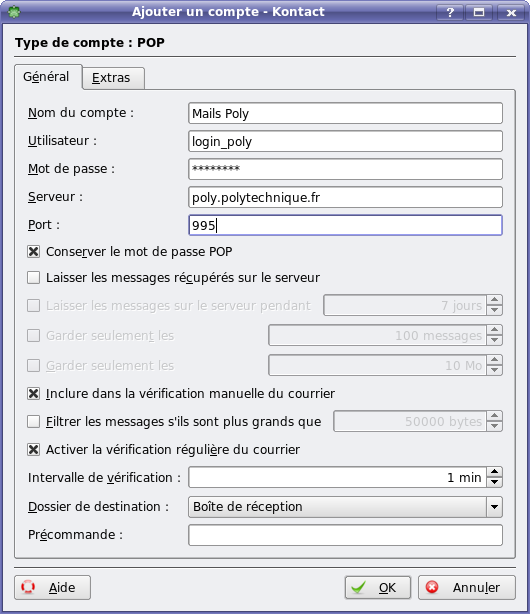
\includegraphics[width=0.48\textwidth]{images/nux_config_kmail_pop} }
      \hspace{\stretch{1}}
      \subfloat[Envoi des messages]{ 
 		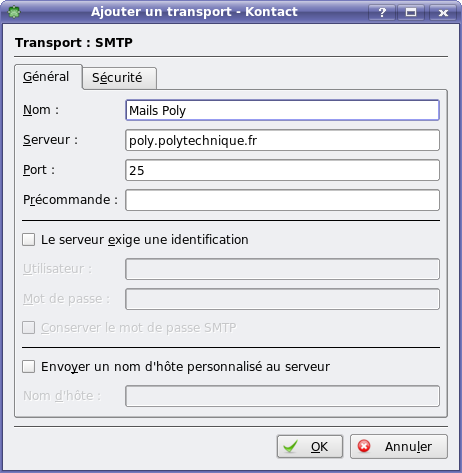
\includegraphics[width=0.48 \textwidth]{images/nux_config_kmail_smtp} }
         	 \caption{Configuration sous \app{Kmail}}
    \end{center}
  \end{figure*}


Utilise les param\`etres suivants pour configurer l'onglet \menu{G\'en\'eral} :
\begin{description}
  \item[Nom] le nom du compte, par exemple : Mails Poly
  \item[Utilisateur] rentre le \emph{login} \server{poly} que t'a fourni la DSI \`a  ton arriv\'ee sur le plateau
  \item[Mot de passe] et l\`a  le mot de passe \server{poly}
  \item[Serveur] \server{poly.polytechnique.fr}
  \item[Port] 995
\end{description}
Ensuite, va dans l'onglet \menu{Extras} et coche la case
\menu{Utiliser SSL pour s\'ecuriser les t\'el\'echargements}.

Maintenant, dans l'onglet \menu{Envoi des messages} clique sur le
bouton \menu{Ajouter\ldots}. Utilise les param\`etres suivants pour le
configurer :
\begin{description}
  \item[Nom] le m\^eme nom de compte que pr\'ec\'edemment
  \item[Serveur] \server{poly.polytechnique.fr}
  \item[Port] 25
\end{description}
Sinon, laisse toutes les cases d\'ecoch\'ees.

%Tu peux aussi configurer l'acc\`es \`a  \app{l'annuaire LDAP} de l'\'Ecole, sorte de carnet d'adresses en ligne qui contient les adresses \emph{mail} de tout le monde sur le campus. Pour ce faire, commence par ouvrir \menu{Outils}, \menu{Carnet d'adresses}, puis va dans \menu{Configuration}, \menu{Configurer kAdressBook}, \menu{Consultation LDAP}. Clique ensuite sur \menu{Ajouter un h\^ote}, et configure comme suit: \\
%\smallskip
%\begin{minipage}[t]{0.48\textwidth}
%\begin{description}
%  \item[H\^ote] \server{ldap.eleves.polytechnique.fr}
%  \item[Port] 389
%  \item[Version de LDAP] 3
%\end{description}  
%\end{minipage} 
%\begin{minipage}[t]{0.48\textwidth}
%\begin{description}  
%  \item[DN] \server{dc=polytechnique, dc=ldap, dc=eleves, dc=fr}
%  \item[S\'ecurit\'e] Non
%  \item[Identification] Anonyme
%\end{description}
%\end{minipage} \\
%Une fois revenu dans \menu{Configuration LDAP}, coche la case \server{ldap.eleves.polytechnique.fr}. Tu as maintenant acc\`es \`a  l'annuaire LDAP lors de la
%r\'edaction de messages, avec tout au plus un red\'emarrage de \app{Kmail}. 
%
%\imagepos{images/nux_config_ldap}{0.55}{Configuration de l'annuaire LDAP sous Kmail}{pht}
%\imagepos{images/nux_config_knode}{0.45}{Configuration de Knode}{ht}
%
%\noindent
%  \begin{figure*}[!h]
%    \begin{center}  
%      \subfloat[Configuration de l'annuaire LDAP sous Kmail]{ 
%      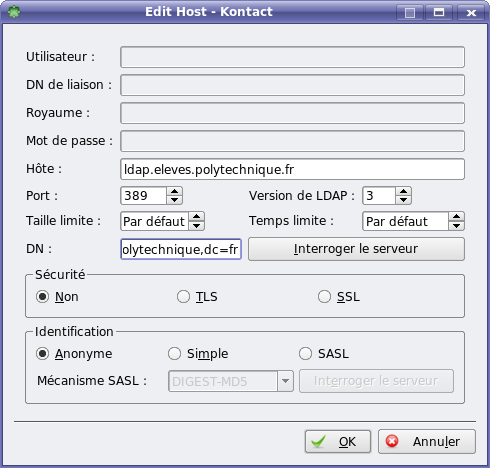
\includegraphics[width=0.48\textwidth]{images/nux_config_ldap}}
%      \hspace{\stretch{1}}
%      \subfloat[Configuration de Knode]{ 
% 		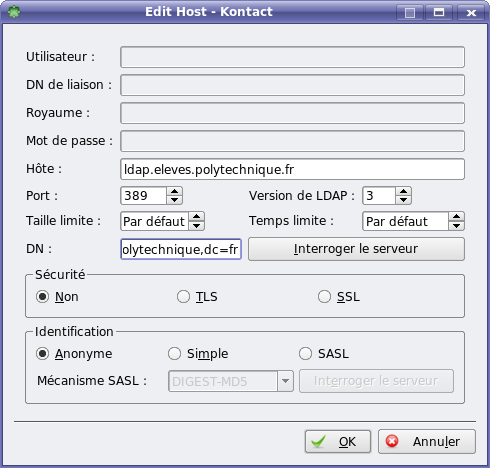
\includegraphics[width=0.48 \textwidth]{images/nux_config_ldap} }
%	\caption{Configurations LDAP et \emph{news}}
%    \end{center}
% \end{figure*}



%\subsubsection{Configuration \emph{news}}
%
%\flimage{images/nux_knode_icon}{0.12}{l} Le client \emph{news} le plus utilis\'e est \app{Knode}. Parmi les autres clients \emph{news}, citons 
%\app{Thunderbird}, \app{Pan} ou \app{slrn}. Ici aussi, la configuration est presque ind\'ependante du logiciel choisi.
%
%
%Sous \app{Knode}, c'est dans le menu \menu{Configuration}, puis \menu{Configurer Knode}. Va dans la rubrique \menu{Comptes, Forums de discussion} et
%cr\'ee un compte en cliquant sur \menu{Ajouter\ldots}.
%
%\imagepos{images/nux_config_knode}{0.45}{Configuration de Knode}{ht}
%
%\pagebreak
%
%Remplis l'onglet \menu{Serveur} avec les informations suivantes :
%\begin{description}
%  \item[Nom] ce que tu veux pour d\'ecrire ce compte, par exemple 'News Frankiz'
%  \item[Serveur] \server{news}
%\nopagebreak  \item[Port] 119
%\end{description}
%
%\pagebreak
% 
%Ensuite occupe-toi de l'onglet \menu{Identit\'e} :
%\begin{description}
%  \item[Nom] mets ton pseudo dans ce champ
%  \item[Organisation] X, \'Ecole polytechnique, comme tu le sens
%  \item[Adresse \'electronique] ton adresse \emph{mail}, pour que les gens puissent te r\'epondre par \emph{mail}.
%\end{description}
%
%Enfin, pour que \app{Knode} puisse envoyer des \emph{mails}, il faut aller
%dans la rubrique \menu{Comptes}, sous-rubrique \menu{Serveur de
%courrier (SMTP)}, et choisir comme serveur d'envoi de \emph{mails}
%\server{poly.polytechnique.fr}, port 25 --- c'est exactement la m\^eme
%configuration SMTP que \app{Kmail}.
%
%Si tu veux mettre une signature \`a  la fin des messages que tu
%posteras, il te suffit de la mettre dans l'onglet \menu{Identit\'e}.
%Sur la plupart des clients la signature est interpr\'et\'ee comme
%ext\'erieure au message et n'est en particulier pas incluse dans le
%texte cit\'e lorsque tu r\'eponds \`a  un message. Pour d\'efinir une
%signature \`a  la main, il suffit de mettre \verb*+-- +\ (c'est \`a  dire
%-{}-<espace>) sur une ligne, et tout ce qui suivra cette ligne
%composera ta signature.
%
%Il ne te reste plus qu'\`a  t'inscrire \`a  des \emph{newsgroups} (reporte-toi \`a  la page \pageref{newsgroups} pour plus d'infos) et \`a  poster ! \\
%
%Pour te connecter aux serveurs de \emph{news} de Polytechnique.org, qui ont un acc\`es s\'ecuris\'e, avec \app{Knode}, il y a une petite subtilit\'e car il
%ne g\`ere pas le SSL. Il faut installer \app{stunnel} qui permet de d\'efinir une redirection SSL de port. Dans \file{/etc/stunnel.conf} (ou parfois \file{/etc/stunnel/stunnel.conf}), mets les lignes suivantes (les trois premi\`eres y sont en principe d\'ej\`a ) :
%\cmdline{\# location of pid file\\
%pid = /etc/stunnel/stunnel.pid\\
%\\
%\# user to run as\\
%setuid = stunnel\\
%setgid = stunnel\\
%\\
%\# Use it for client mode\\
%client = yes\\
%\\
%\# sample service-level configuration\\
%{[}nntps{]}\\
%accept  = 1119\\
%connect = ssl.polytechnique.org:563\\
%TIMEOUTclose = 0
%}
%
%Il ne te reste plus qu'\`a  lancer \app{stunnel} par :
%\cmdline{/etc/init.d/stunnel start}
%
%Et tu peux ainsi lire les \emph{news} de Polytechnique.org en mettant \server{localhost} comme serveur et
%\server{1119} comme port. Il faut aussi que tu coches \menu{Le serveur exige une identification} et
%que tu rentres ton nom d'utilisateur \`a  Polytechnique.org et ton mot de passe, que tu peux d\'efinir
%sur \urllink{https://www.polytechnique.org/Xorg/SMTPSecurise}.

\clearpage
